% --------------------------------------------------------------
% This is all preamble stuff that you don't have to worry about.
% Head down to where it says "Start here"
% --------------------------------------------------------------

\documentclass[12pt]{article}

\usepackage[margin=1in]{geometry}
\usepackage{amsmath,amsthm,amssymb}
\usepackage{graphicx} %This allows to include eps figures
\usepackage{subcaption}
\usepackage[section]{placeins}
\usepackage{layout}
\usepackage{etoolbox}
\usepackage{mathabx}
\usepackage{animate}
\usepackage{array}
% This is to include code
\usepackage{listings}
\usepackage{xcolor}
\definecolor{dkgreen}{rgb}{0,0.6,0}
\definecolor{gray}{rgb}{0.5,0.5,0.5}
\definecolor{mauve}{rgb}{0.58,0,0.82}
\lstdefinestyle{Python}{
    language        = Python,
    basicstyle      = \ttfamily,
    keywordstyle    = \color{blue},
    keywordstyle    = [2] \color{teal}, % just to check that it works
    stringstyle     = \color{green},
    commentstyle    = \color{red}\ttfamily
}

\newenvironment{conditions}
  {\par\vspace{\abovedisplayskip}\noindent\begin{tabular}{>{$}l<{$} @{${}={}$} l}}
  {\end{tabular}\par\vspace{\belowdisplayskip}}

\newcommand{\N}{\mathbb{N}}
\newcommand{\Z}{\mathbb{Z}}

\newenvironment{theorem}[2][Theorem]{\begin{trivlist}
\item[\hskip \labelsep {\bfseries #1}\hskip \labelsep {\bfseries #2.}]}{\end{trivlist}}
\newenvironment{lemma}[2][Lemma]{\begin{trivlist}
\item[\hskip \labelsep {\bfseries #1}\hskip \labelsep {\bfseries #2.}]}{\end{trivlist}}
\newenvironment{exercise}[2][Exercise]{\begin{trivlist}
\item[\hskip \labelsep {\bfseries #1}\hskip \labelsep {\bfseries #2.}]}{\end{trivlist}}
\newenvironment{reflection}[2][Reflection]{\begin{trivlist}
\item[\hskip \labelsep {\bfseries #1}\hskip \labelsep {\bfseries #2.}]}{\end{trivlist}}
\newenvironment{proposition}[2][Proposition]{\begin{trivlist}
\item[\hskip \labelsep {\bfseries #1}\hskip \labelsep {\bfseries #2.}]}{\end{trivlist}}
\newenvironment{corollary}[2][Corollary]{\begin{trivlist}
\item[\hskip \labelsep {\bfseries #1}\hskip \labelsep {\bfseries #2.}]}{\end{trivlist}}



\begin{document}

% --------------------------------------------------------------
%                         Start here
% --------------------------------------------------------------

%\renewcommand{\qedsymbol}{\filledbox}

\title{Assignment 6}%replace X with the appropriate number
\author{Nalet Meinen and Pascal Wyss\\ %replace with your name
Finite Element Analysis I
}
\maketitle

\begin{figure}[!htb]
  \centering
  \vspace*{1cm}
  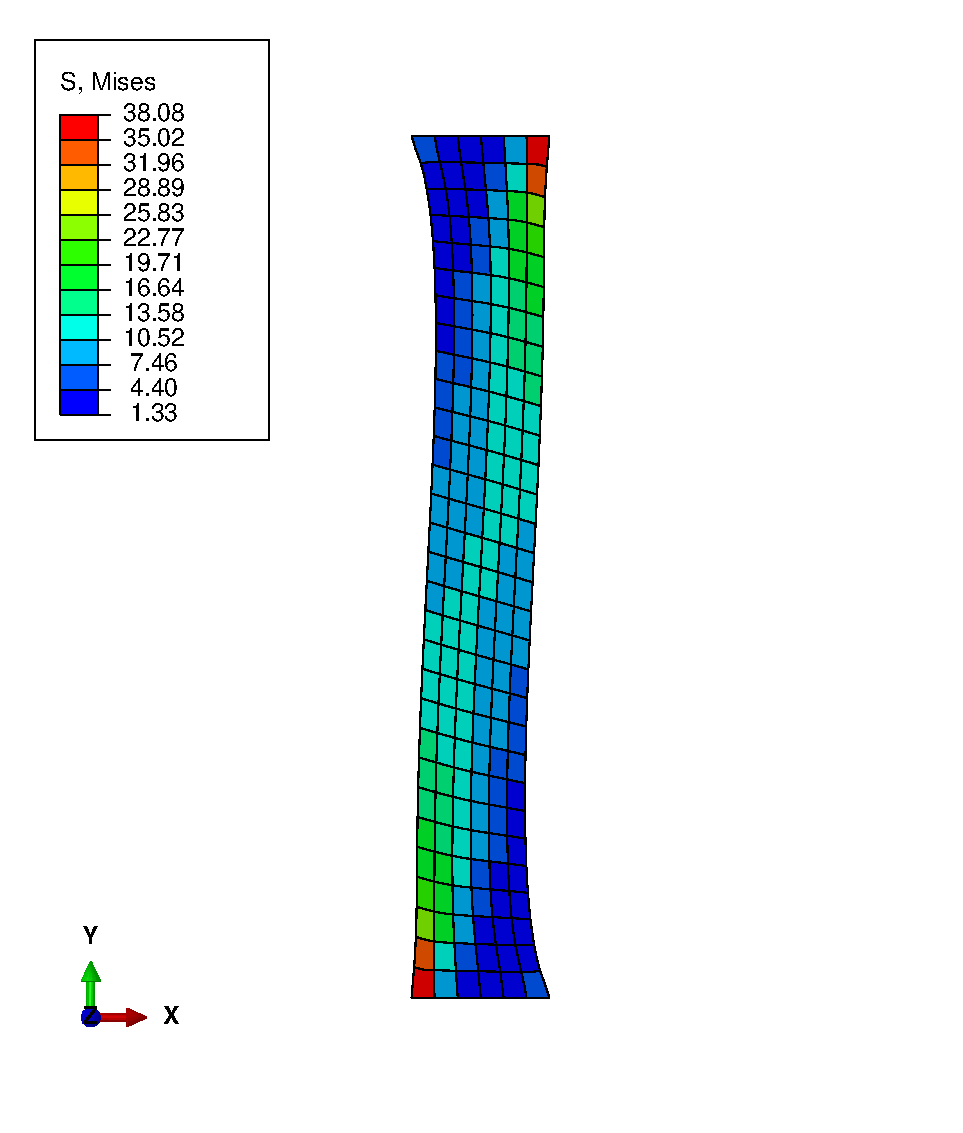
\includegraphics[trim={50mm 20mm 50mm 20mm},clip,width=0.35\linewidth]{pics/s_mises_30}
  \label{fig:0}
\end{figure}

\newpage

\section*{Abstract}
The objective of this assignment is to determine the material parameters. The data is gathered via an anatomical sample during experimental measurements. However, the material parameters cannot be so easily determined by the experimental data. So further analysis is necessary to get a better numerical model that later can be used for further analyzing.
This assignment analyzes the material from the cornea, a part of the eye. The numerical model should give a better understanding of the fibers in the cornea and how they are reacting due to exposes of stresses.


\tableofcontents
\pagebreak
\section{Introduction}
In this assignment, we will create a model that should mimic a part of the cornea. The material of the model in Abaqus should have anisotropic and hyperelastic properties. A good fit for describing this behavior can be made with the Holzapfel-Gasser-Ogden function, which describes very well the strain energy potential with collagen fibers.
What we are doing is gathering control data from actual experiments in the lab. Therefore a part of the cornea is exposed to force, which generates stresses on the sample of tissue. we are measuring the displacement which happens on a specific force. with that data, a model can be created in Abaqus with the Holzapfel-Gasser-Ogden function. However, the function is based on parameters which we don't know yet, but can only guess.
\begin{equation}\label{eq:holzapfel}
  W=C_{10}(\Bar{I}_{1}-3)+\frac{1}{D}\Big(\frac{J^{2}-1}{2}-\ln J\Big)+\frac{k_{1}}{2k_{2}}\sum_{\alpha=1}^{N}(\exp[k_{2}<E_{\alpha}>^{2}]-1)
\end{equation}
\begin{equation}\label{eq:holzapfel_e}
  E_{\alpha}=\kappa(I_{3}-3)+(1-3\kappa)(I_{4(\alpha)})
\end{equation}
\begin{conditions}
  W                             &  strain energy per unit of reference volume\\
  C_{10},D,k_{1},k_{1},k        &  are temperature-dependent material parameters\\
  N                             &  is the number of families of fibers ($N \leq 3$)\\   
  \Bar{I}_{1}                   &  is the first invariant of $\Bar{C}$ \cite{Holzapfel-Gasser-Ogden} \\
  J                             &  is the elastic volume ratio\\
  I_{4(\alpha)}                 &  are pseudo-invariants of $\Bar{C}$
\end{conditions}
Giving this information from the Abaqus documentation \cite{Holzapfel-Gasser-Ogden} and knowing that is a good fit for the modeling of collagen fibers, a sample can now be created.
\newpage
\section{Methods}

\subsection{Sample and experimental data}

We created a model with CPS4R mesh type. Based on the last assignments, the reduced integration
gave us the best result, so we stick with that.

% \begin{figure}[!htb]
%   \centering
%   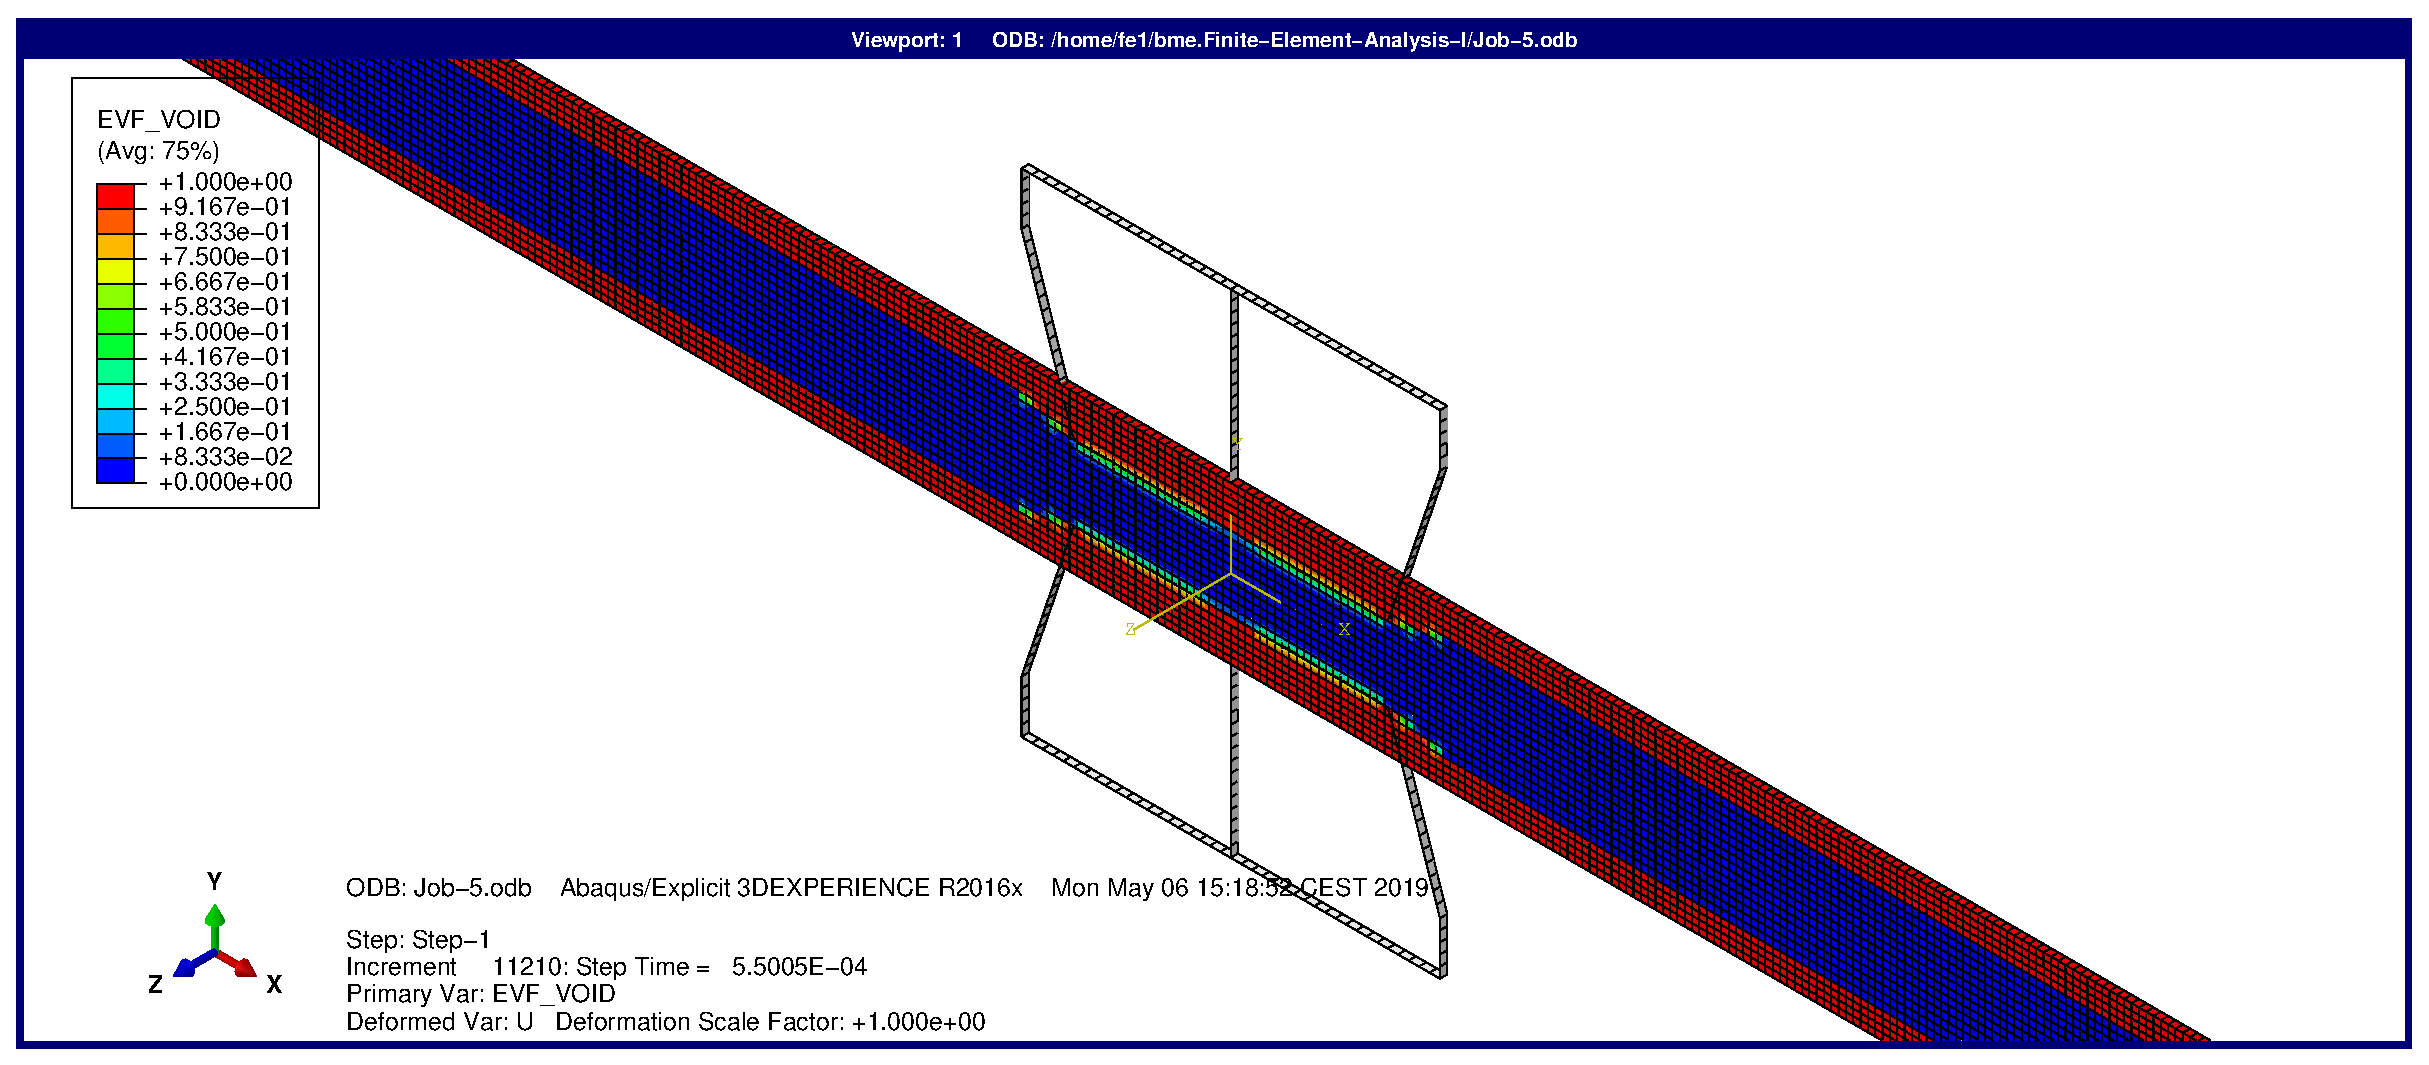
\includegraphics[width=0.9\linewidth]{pics/sexy3Dbild}
%   \caption{Node to node with no sliding}
%   \label{fig:2}
% \end{figure}

% \begin{figure}[!htb]
%   \centering
%   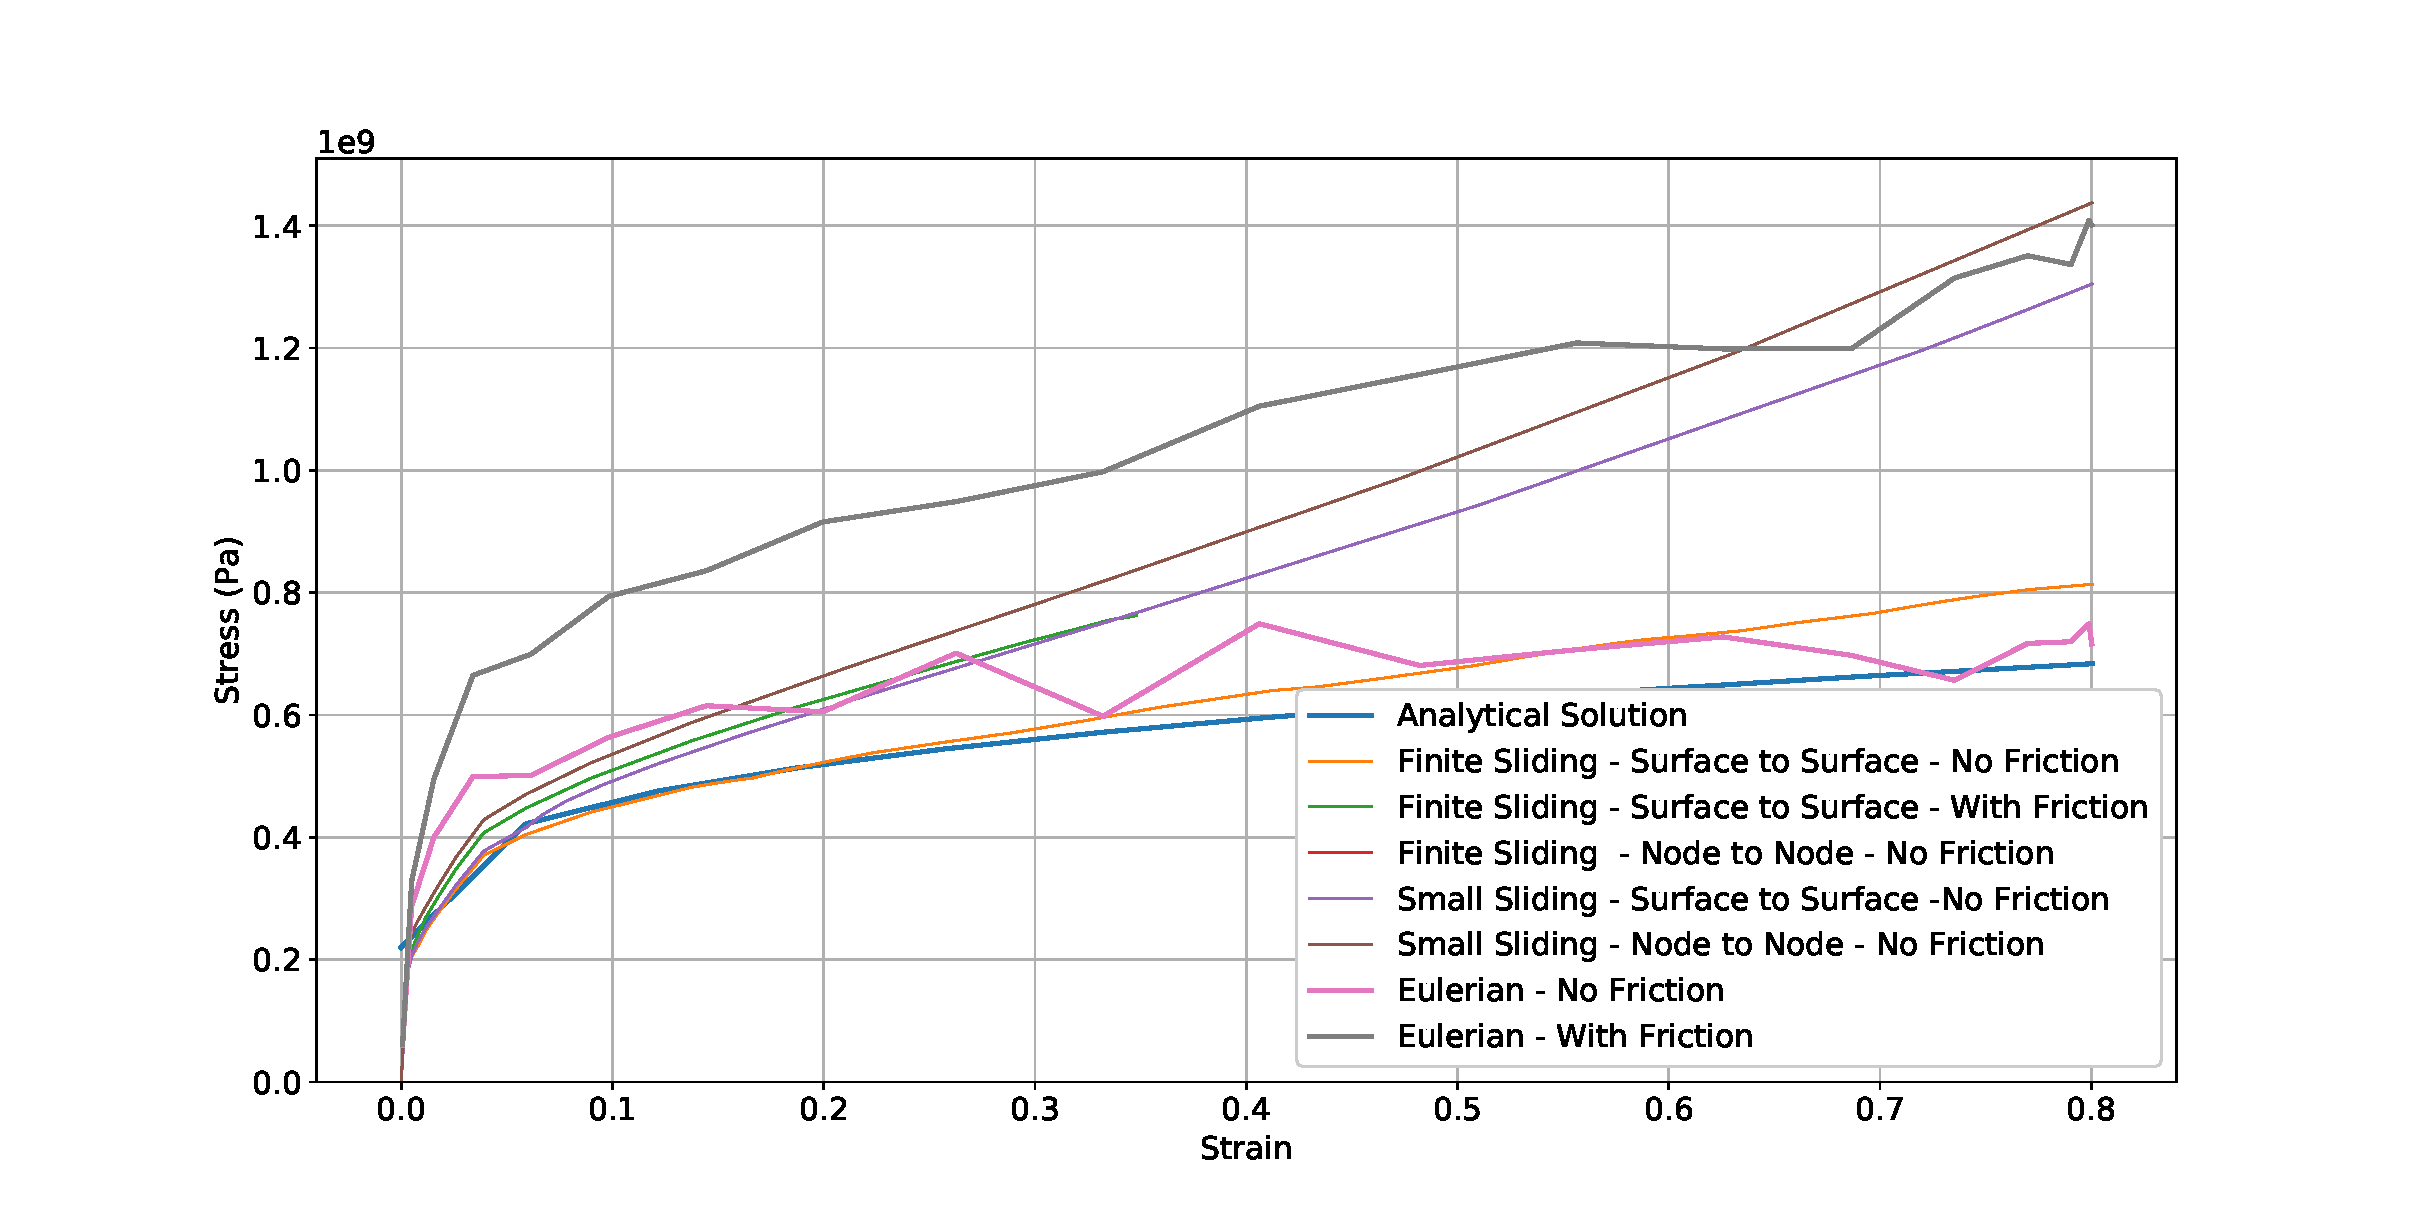
\includegraphics[width=0.9\linewidth]{pics/analytical_compared_euler}
%   \caption{Result of the previous assignment with eulerian result}
%   \label{fig:3}
% \end{figure}


\pagebreak
\section{Results and Discussion}

The analytical and the experimental results are similar.
Logically the experiment with introduced friction (friciton coefficien 0.2) results in a higher
stress/strain ration, as energy of the compression gets lost in friction. 
during modelling, we ran into troubles with the simulation due to the sharp corner of the press.
Thus we introduced a small 1mm fillet to smoothen the process. This worked out fine and the results 
got better and were calculated more quickly.

The stress/strain ratio calculations which allowed for small sliding show a higher stress per strain ratio.


\pagebreak
\begin{thebibliography}{9}
  \bibitem{Holzapfel-Gasser-Ogden} 
  https://www.sharcnet.ca/Software/Abaqus610/Documentation/docs/v6.10/books/stm/default.htm?startat=ch04s06ath125.html\#stm-mat-anisohyperelastic-holzapfel
\end{thebibliography}


\end{document}